\chapter{Indici di posizione}
\label{cha:Indicidiposizione}
\begin{center}
		\includestandalone[width=\linewidth]{grafici/indicigrafico}
\end{center}

\begin{table}
	\centering
	\begin{tabular}{S[table-format=1.0]S[table-format=2.0]S[table-format=3.0]}
		\toprule
		{$x_{i}$}&{$n_{i} $}  &{$x_{i}\cdot n_{i}$}  \\ 
		\midrule
		6	& 8 & 48 \\
		3	&  6&  18\\ 
		4	&  5& 20 \\ 
		5	&  3& 15 \\
		\midrule 
		{Totali}	&22&  101  \\
		\bottomrule 
	\end{tabular} 
	\caption{Media aritmetica ponderata}
	\label{tab:MediaAritmteicaPonderata}
\end{table}
\section{Medie}
Il concetto di media aritmetica dovrebbe essere noto, nel seguito daremo alcune definizioni che dipenderanno anche da quanto è stato detto nel capitolo precedente.
\begin{defn}[Media aritmetica]
	Se abbiamo un insieme di dati $\lbrace x_{1},x_{2},x_{3},\cdots,x_{n}\rbrace$ la media aritmetica\index{Media!aritmetica} $M$ di questi valori  è  la somma dei valori diviso il numero di elementi.\[M=\dfrac{x_{1}+x_{2}+x_{3}+\cdots+x_{n}}{n}=\dfrac{\sum_{i=1}^{n}x_{i}}{n} \]
\end{defn}

Nel caso di mentre un insieme  di frequenze assolute avremo la definizione:
\begin{defn}[Media aritmetica ponderata]
Se abbiamo una distribuzione di frequenze di n dati $\lbrace x_{1},x_{2},x_{3},\cdots,x_{n}\rbrace$ e un valore $x_{i}$ compare $n_{i}$ volte,  allora la media aritmetica ponderata\index{Media!aritmetica!ponderata}  $M$ dei valori è: \[M=\dfrac{x_{1}\cdot n_{1}+x_{2}\cdot n_{2}+\cdots+x_{n}\cdot n_{n}}{n_{1}+n_{2}+\cdots+n_{n} }=\dfrac{\sum_{i=1}^{n}x_{i}\cdot n_{i}}{\sum_{i=1}^{n} n_{i}}=\dfrac{\sum_{i=1}^{n}x_{i}\cdot n_{i}}{n}\]
\end{defn}
Il calcolo della media aritmetica non porta a grossi problemi, supponiamo di avere otto misure di velocità \[x_{i}=\SIlist[list-separator = {;}]{4.2;3.4;2.3;5.4;3.4;3.5;4.3;3.3}{\metre\per\second}\] La media $M$ è \[M=\dfrac{\num{4.2}+\num{3.4}+\num{2.3}+\num{5.4}+\num{3.4}+\num{3.5}+\num{4.3}+\num{3.3}} {8}=\SI{3.725}{\metre\per\second}\]

Per calcolare la media ponderata possiamo seguire il seguente esempio. La tabella riporta dei dati di un esperimento assieme alle frequenze assolute con cui essi compaiono. 
\begin{center}
\begin{tabular}{l*{4} {S[table-format=1.0]}}
	{$x_{i}=$}	&6  &3  &4  &5  \\
	\midrule 
	{$n_{i}=$}	& 8 &6  & 5 & 3 \\ 
\end{tabular}
\end{center}
Costruiamo ora  la~\vref{tab:MediaAritmteicaPonderata}.

Sommando l'ultima colonna della tabella otteniamo la media aritmetica ponderata segue 
\[M=\dfrac{\sum_{i=1}^{q}x_{i}\cdot n_{i}}{n}=\dfrac{\num{101}}{\num{22}} \approx\num{4.590} \]
La~\vref{tab:MediaAritmteicaPonderataExcel} permette di riprodurre l'esempio.

\section{Moda}
\begin{defn}[Moda]
	Data una distribuzione di dati, la moda\index{Moda} è il valore che si presenta con più frequenza.
\end{defn}
Poniamo di avere la seguente distribuzione di dati
\begin{center}
	\begin{tabular}{l*{5} {S[table-format=1.0]}}
		{$x_{i}=$}	&2  &7  &8  &3  &5 \\
		\midrule 
		{$n_{i}=$}	& 6 &8  & 5 & 10 & 2\\   
	\end{tabular}
\end{center}
\begin{figure}
	\centering
	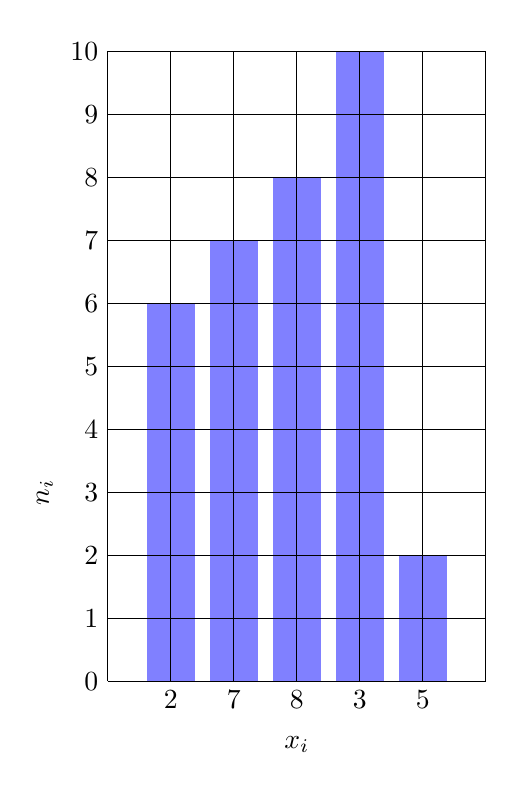
\begin{tikzpicture}[scale=0.8]
	\draw[line width=6mm,color=blue!50] plot[ycomb] coordinates{(1,6) (2,7) (3,8) (4,10)
		(5,2)};
	\draw (0,0) grid (6,10);
	\foreach \y in {0,1,...,10} \draw(0,\y)node[left]{\y};
	\foreach \n/\x in {5/5,3/4,8/3,7/2,2/1}
	\draw (\x,0) node [below] {\n};
	%\foreach \x in {1,2,...,10} \draw(\x,0)node[below]{\x};
	\draw (3,-1) node{$x_i$};
	\draw (-1,3) node[rotate=90]{$n_i$};
	\end{tikzpicture}
	\caption{Moda}
	\label{fig:Moda}
\end{figure}
Come si vede dal grafico~\vref{fig:Moda} il massimo numero di frequenze è per $n_i=10$ quindi la moda $M_o=3$. La moda non è sempre unica per esempio 
se abbiamo la seguente distribuzione di dati
\begin{center}
	\begin{tabular}{l*{5} {S[table-format=1.0]}}
		{$x_{i}=$}	&7  &3  &2  &4  &5 \\
		\midrule 
		{$n_{i}=$}	& 4 &2  & 3 & 4 & 2\\   
	\end{tabular}
\end{center}
Le frequenze massime sono due e sono per $n_i=4$ e le mode sono due $M_o=4$ e $M_o=4$ cioè si dice che le distribuzioni sono bimodali\index{Distrubuzione!bimodale} come appare nel grafico~\vref{fig:BiModale}
\begin{figure}
	\centering
	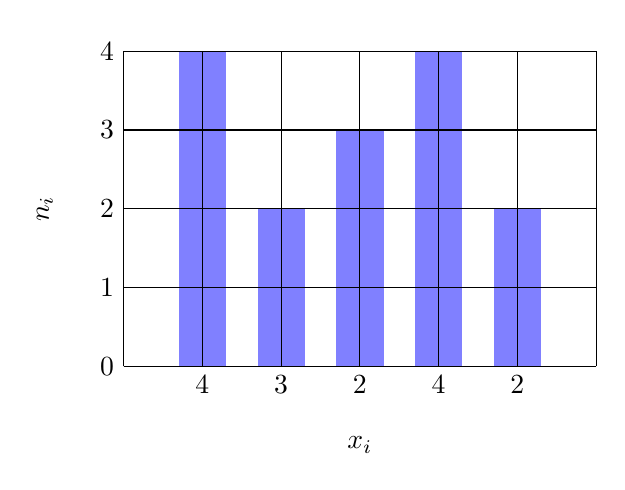
\begin{tikzpicture}%[scale=0.8]
	\draw[line width=6mm,color=blue!50] plot[ycomb] coordinates{(1,4) (2,2) (3,3) (4,4)
		(5,2)};
	\draw (0,0) grid (6,4);
	\foreach \y in {0,1,...,4} \draw(0,\y)node[left]{\y};
	\foreach \n/\x in {2/5,4/4,2/3,3/2,4/1}
	\draw (\x,0) node [below] {\n};
	%\foreach \x in {1,2,...,10} \draw(\x,0)node[below]{\x};
	\draw (3,-1) node{$x_i$};
	\draw (-1,2) node[rotate=90]{$n_i$};
	\end{tikzpicture}
	\caption{Bimodale}
	\label{fig:BiModale}
\end{figure}
\section{Mediana}
\begin{defn}[Mediana]
	Dato un inseme ordinato di valori, la mediana\index{Mediana}  ha tanti dati che la precedono quanti quelli che la seguono.
\end{defn}
Per determinare la mediana $M_e$ ordiniamo i dati in modo che $x_1\leq x_2\leq\cdots\leq x_n $. Abbiamo due casi in: i valori sono in numero dispari o i dati sono in in numero pari. Nel primo caso allora la mediana è il valore di posto $k=\dfrac{n-1}{2}+1=\dfrac{n+1}{2}$. 

Praticamente se vi sopo per esempio undici valori e li ordiniamo dal più piccolo al più grande, l'elemento di posto $ \dfrac{11+1}{2}=6$ è l'elemento che cerchiamo. Quel valore ha cinque elementi prima e cinque dopo. Se il numero totale  degli elementi è pari, non vi è un elemento centrale. In questo caso di poniamo  per convenzione che se $k=\dfrac{n}{2}$ $M_e=\dfrac{x_k+x_{k+1}}{2}$

